\section{Benefits and Challenges using LOD (RQ2 \& RQ3)}~\label{section:benefits}
As mentioned in the introduction, we identified \textit{students}, \textit{researchers} and \textit{administration employees} as import stakeholders at a university. This chapter describes the methodology and results of the conducted case study involing researcher. The essential question of the case study was RQ2 (``\textit{What are major benefits and barriers for each stakeholder and what are useful use cases?}'') and RQ3 (``\textit{What are major challenges for the implementation of a Linked Open Data solution?}'') 
A case study concerning students was conducted by Kevin Haller~\cite{article:haller_publishing_2016} and another one concerning administration employees by Stefan Gamerith~\cite{article:gamerith_publishing_2016}.

The first section of this chapter describes the applied methodology (see section~\ref{subsection:methodology}). The second section evaluates and analyzes the results of the case study, investigating the possible benefits, barriers and challenges of some use cases and a general view at the interviewees (see section~\ref{subsection:results}).

\subsection{Methodology}
In this study the data were acquired by a coordinated set of semi-structured interviews. As mentioned the stakeholders were classified into three groups (\textit{administrative staff}, \textit{students} and \textit{researchers}) and therefore three different versions of the questionnaire but with joint parts for statistically evaluation were worked out. For each version exists an according paper, in this work only the category "`researcher"' will be described.

\subsubsection{Design of questionnaire}
The main purpose of the interviews were the collecting of the stakeholders thoughts, needs and knowledge, so the method of of a semi-structured interview was chosen. A \textit{fully structured interview} would not be adequate because of it's strict character allowing only predefined answers and a \textit{unstructured interview} would be to difficult to analyze.

After choosing the method, the questionnaire was defined. To allow a general, generic shared analyze of the interviewees the team decided to mix open questions from the semi-structured model with closed questions with fixed, predefined questions. The result had four parts:

\begin{enumerate}
	\item General question about the interviewee for classification, about his/her work
	\item General question about the interviewee's knowledge in general technical and LOD context. This part is the part for statistical evaluation.
	\item Explanation of LD, followed by a specific set of questions targeting the thoughts and opinions of the interviewee about presented use cases and example application. Motivation of this part is to introduce the interviewee to LOD if it is an unknown topic and let him/her start to think about LOD to prepare the next part
	\item Wide open Questions to explore and find use cases and existing data sources for LOD application at the university.
\end{enumerate}

The examples from part 3 were LD in libraries (see~\ref{ld-libraries}) and an obvious source of research related data: the publication database.

\subsubsection{Description of interviewed people}
As mentioned the interviewees of this study were chosen according to the category "`\textit{Research}"', so the interview partner were active researcher in various fields. Altogether four interviews were done. Because of the technical character of LOD the chosen people are all technically experienced so they are able to imagine use cases at the university. In future work there is a need of more less experienced researchers to understand their thoughts.

\subsubsection{Data Validity and Quality}
To ensure both a continuous conversation flow and a high quality recording of the spoken words, the interviews were held in teams, one speaker and one writer making notes. Additional all interviews were audio recorded.
As result the data are available as interview notes and audio records.
\newpage
\subsection{Results}\label{results}
After giving a detailed description of the used methodology in the previous subsection this subsection contains the interviews outcome. First the general questions about the interviewees background are evaluated and interpreted. Because this part was included in all three questionnaires, this part also includes data from the other reports for comparing the data, but only the data from the researcher interviews are interpreted. In the next parts, the use case of the library data and publication data are evaluated and their potential benefits, barriers and disadvantages analyzed. In the last part, the ideas and mentions from the open questions are evaluated.

\subsubsection{General statistically evaluation of the interviewees background}\label{stat_general}

\begin{figure}[htbp]
\centering
\label{Fi:lod-exp}
	\begin{tikzpicture}
		\begin{axis}
			[title=Level of ICT-Expertise,
			ybar,% Balken
			% urspr�ngliche y-Werte unterhalb der Balken:
			nodes near coords,nodes near coords align=above,point meta=rawy,
			axis x line=bottom, axis y line=left,% Achsen nur unten und links,
			%xlabel=blub,ylabel=bla, % Beschriftung der Achsen
			ymin=0,% minimaler y-Wert ist 0
			xtick=data,% xticks nur an Stellen mit Daten
			enlargelimits=auto,% Vergr��ern der R�nder des Diagramms
			% Ausgabe der x Werte ohne Tausendermarkierung@
			x tick label style={/pgf/number format/1000 sep=},
			legend pos=north west]
			\addplot table[x=Question, y=Number] {data/data_general_researcher_1.csv};
			\addplot table[x=Question, y=Number] {data/data_general_students_1.csv};
			\addplot table[x=Question, y=Number] {data/data_general_admin_1.csv};
			\legend{Researcher, Students, Administration}
		\end{axis}
	\end{tikzpicture}
	\begin{tikzpicture}
		\begin{axis}		
			[title=Level of LOD-Expertise,
			ybar,% Balken
			% urspr�ngliche y-Werte unterhalb der Balken:
			nodes near coords,nodes near coords align=above,point meta=rawy,
			axis x line=bottom, axis y line=left,% Achsen nur unten und links,
			%xlabel=blub,ylabel=bla, % Beschriftung der Achsen
			ymin=0,% minimaler y-Wert ist 0
			xtick=data,% xticks nur an Stellen mit Daten
			enlargelimits=auto,% Vergr��ern der R�nder des Diagramms
			% Ausgabe der x Werte ohne Tausendermarkierung@
			x tick label style={/pgf/number format/1000 sep=},
			legend pos=north east]
			\addplot table[x=Question, y=Number] {data/data_general_researcher_2.csv};
			\addplot table[x=Question, y=Number] {data/data_general_students_2.csv};
			\addplot table[x=Question, y=Number] {data/data_general_admin_2.csv};
			\legend{Researcher, Students, Administration}
		\end{axis}
	\end{tikzpicture}
	\caption[Level of Experience]{Level of Experience}
\end{figure}

The first part of the interview aimed to categorize the interview partners and to understand their background. They had to estimate their level of expertise in the field of Information \& Communication Technologies and in the field of Linked Open Data in a formal way and then describe their daily work and responsibilities at the university. This part was identical in all three interview series (administration, students and researcher), so the result can be compared. The levels of expertise can be seen in figure~\ref{Fi:lod-exp} and the according rating scales in table~\ref{table:rating-scales}. For a detailed description of the administration and student interviews see the corresponding reports~\citet{article:gamerith_publishing_2016} (administration data) and ~\citet{article:haller_publishing_2016}(data concerning students).

Tough all four research-interviewees had a high expertise in ICTs, their expertise in LOD are mainly unincisive, although everyone already knew the concept of LOD. This can easily explained by their research fields (see table~\ref{table:interviewee-background}): everyone works in a technical context. 

This could be seen as advantage as well as disadvantage. On the one hand the interviewed persons needed lesser effort to understand the benefits of LOD and could easier imagine further use-cases and possible data sets for LOD. But on the other hand, their perspectives were in some way restricted by their profession - a more divergent angle of view may be interesting for further studies to explore more ``non-technical'' use-cases. But for an initial study like this one it may be enough.

	
\begin{figure}[htbp]
  \centering
	\label{table:rating-scales}
	\begin{tabular}{ c | l  | p{10cm} }
		\textbf{Value} & \textbf{ICT} & \textbf{LOD}\\			\hline
		1 & Fundamental & I never heard of Linked Open Data.\\ \hline		
		2 & Novice & I heard of Linked Open Data, but never used it.\\		\hline
		3 & Intermediate & I used Linked Open Data in a not intense way. E.g. as part of a workshop or home project.\\		\hline
		4 & Advanced & I used Linked Open Data in a practical project.\\		\hline
		5 & Expert & I used Linked Open Data in several practical projects and consider myself an expert in Linked Open Data.\\
	\end{tabular}
	\caption[Rating scales]{Rating scales for the level of expertise in the field of ICT and LOD.}
\end{figure}

\begin{figure}[htbp]
  \centering
	\label{table:interviewee-background}
	\begin{tabular}{ c | l | c }
		\textbf{ID} & \textbf{Assignment} & \textbf{Date of interview} \\ \hline
		A & research \& teaching in HCI & 15.12.2015\\
		B & research in information retrieval & 04.12.2015\\
		C & research transfer & 23.11.2015\\
		D & research in audio and video analysis & 24.11.2016\\
	\end{tabular}
	\caption[Interviewees background]{Background information of the interviewees and the corresponding interviews.}
\end{figure}

\subsubsection{Library data}

\begin{figure}[htbp]
\centering
\subfigure[Homepage and simple search]
{\scalebox{0.3}{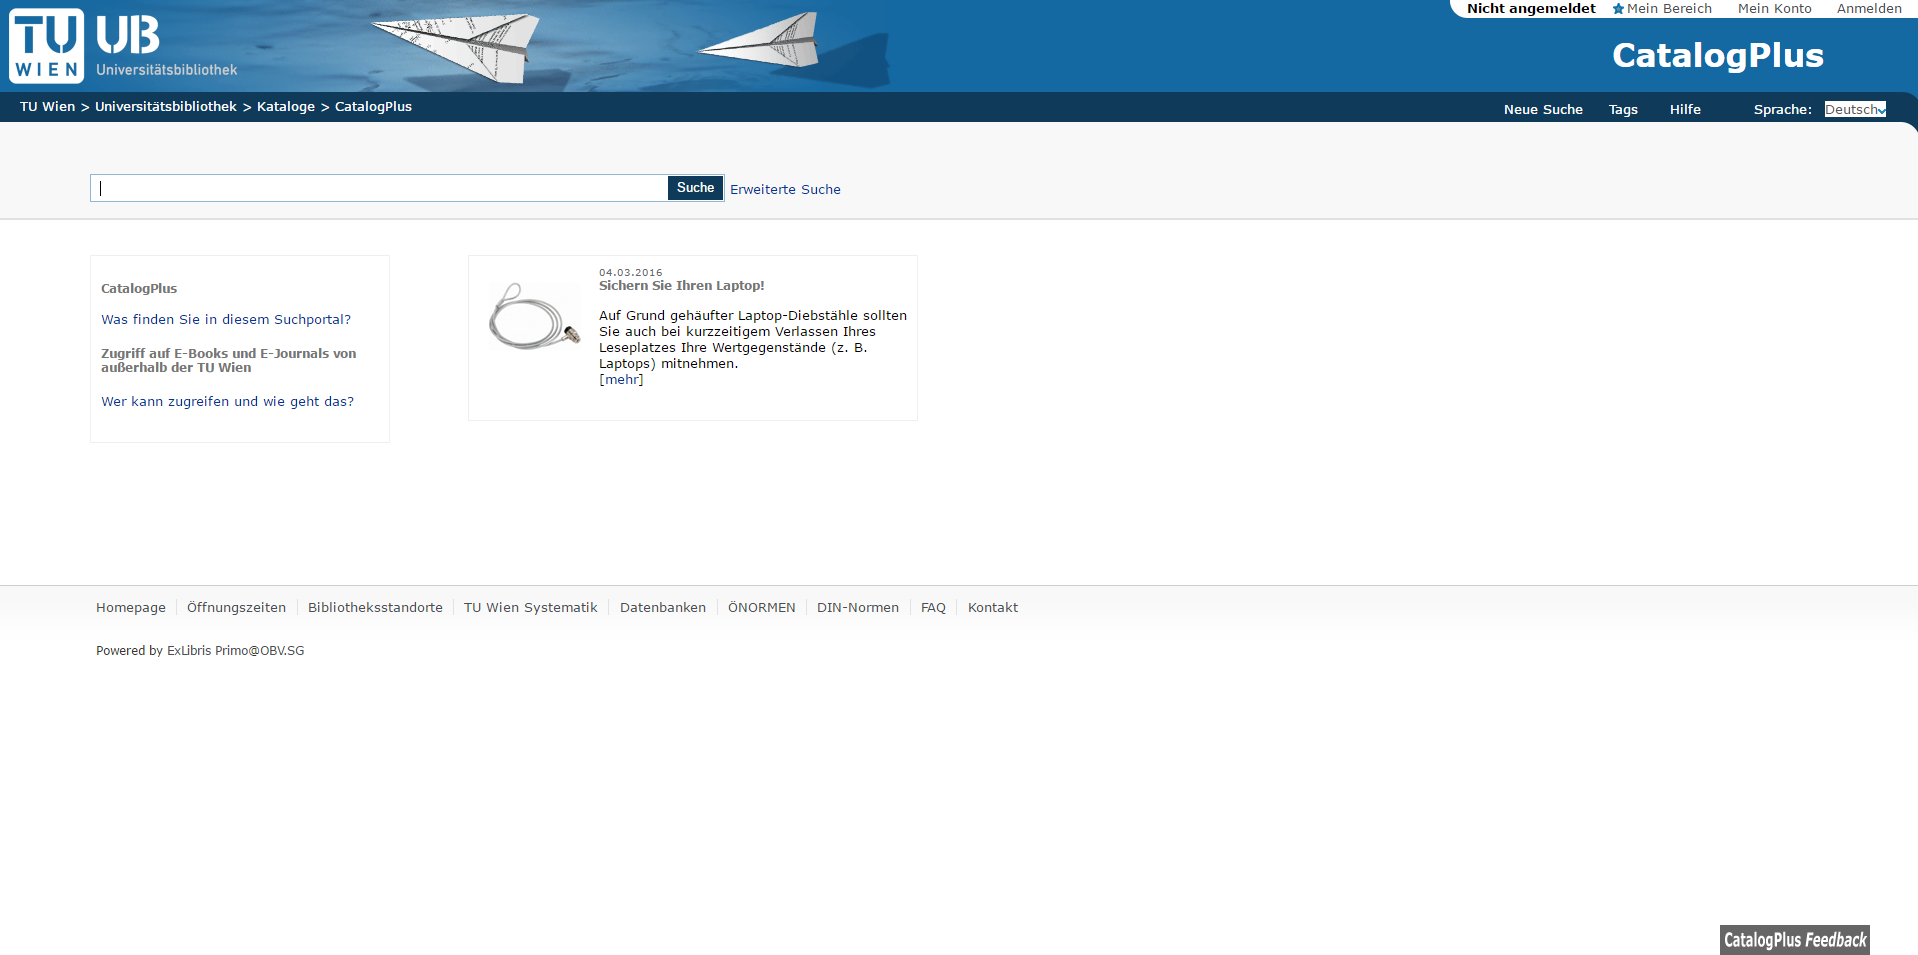
\includegraphics{images/screenshots/screenshot_ub_tu.PNG}}}
\subfigure[Extended search]
{\scalebox{0.3}{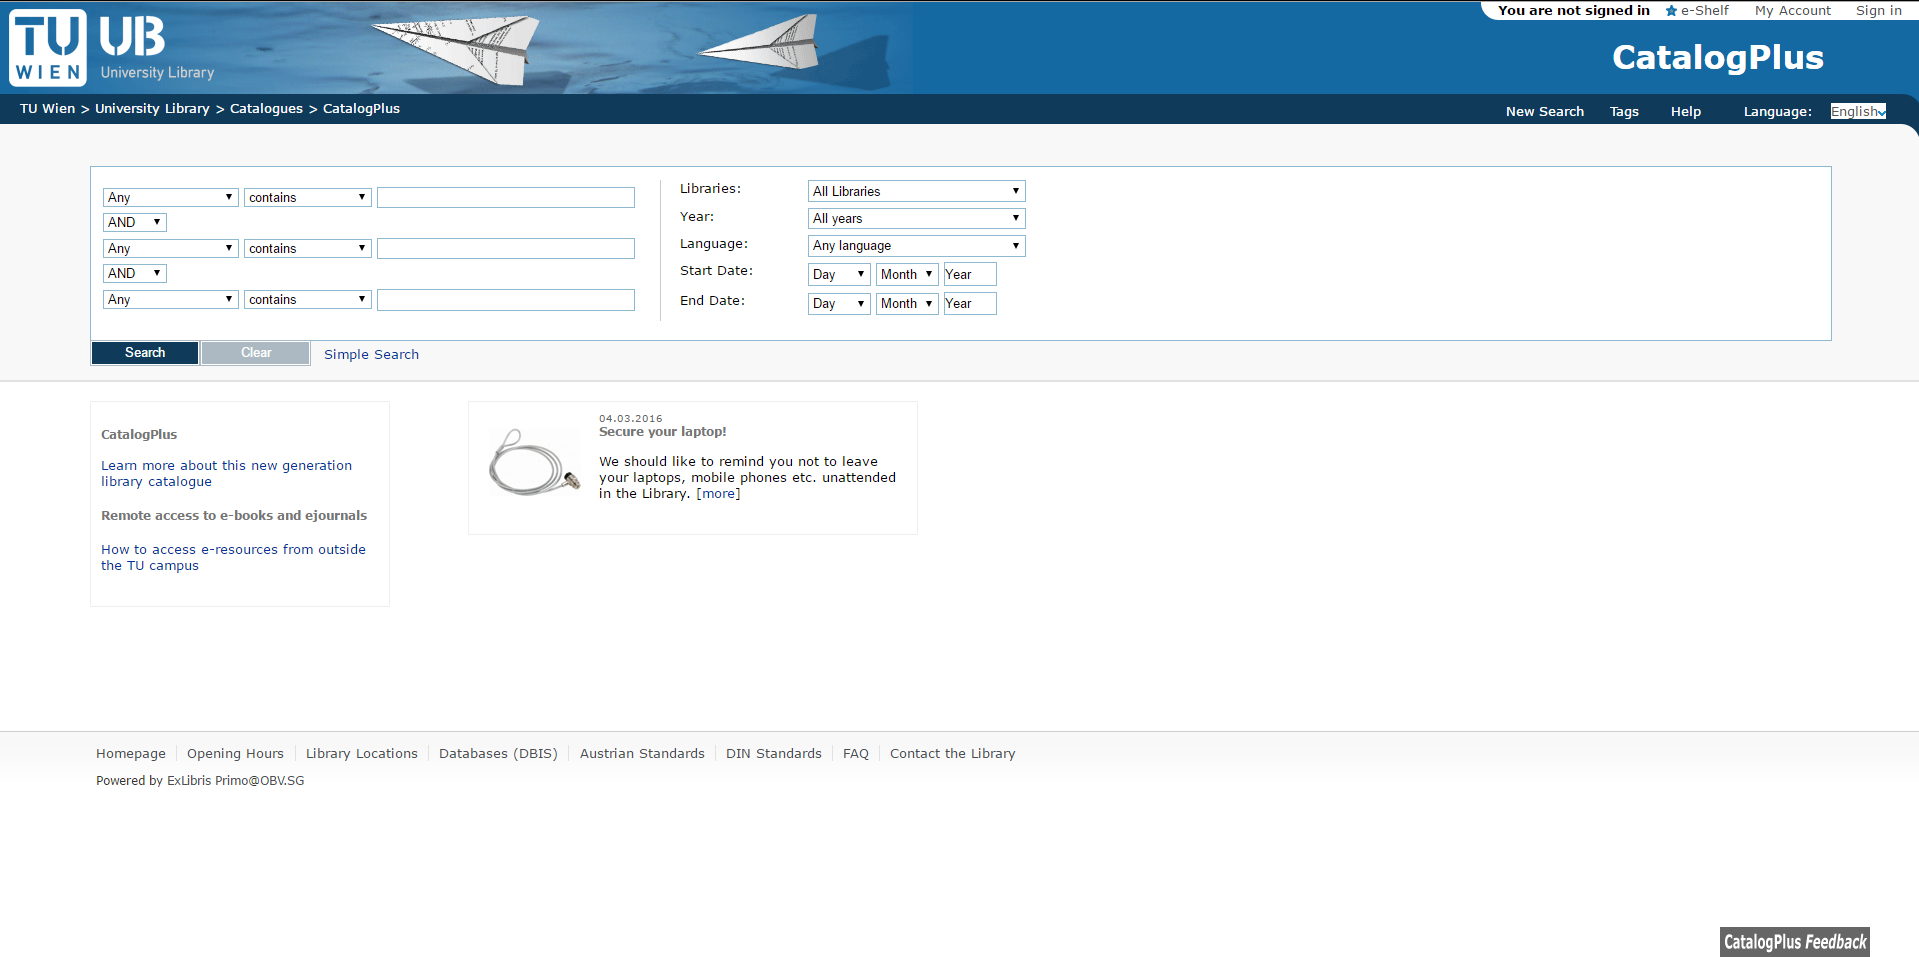
\includegraphics{images/screenshots/screenshot_ub_tu_extended_search.PNG}}}
\caption[Website of the TUVienna library]{Website of the TUVienna library}
\label{Fi:UB_TU}
\end{figure}

\paragraph{Use case}
This question aimed for a use case similar to the project Linked Data Libraries (described in Section ~\ref{ld-libraries}). The proposed scenarios was to publish the data or meta-data of the university library (and all of its specialized libraries) as LOD and provide an application to access the data. A further option of this scenario would be an interlinking to other LOD data sets, e.g. from the publisher ``Springer'' or to other universities like LD4L do it.

\paragraph{Statistically evaluation}
It can be seen in Figure~\ref{Fi:lib-data} that the interviewed persons strongly agreed to the scenario (found it ``extremely useful'') and could imagine a similar project at the TU Vienna. Only one interviewee found it difficult to see advantages and therefore argued that he wouldn't use it. Another one found it indeed useful in a general context but not for his own work.

\begin{figure}[htbp]
\centering
	\begin{tikzpicture}
		\begin{axis}		
			[title=Usefulness of library (meta-)data as LOD,
			ybar,% Balken
			% urspr�ngliche y-Werte unterhalb der Balken:
			nodes near coords,nodes near coords align=above,point meta=rawy,
			axis x line=bottom, axis y line=left,% Achsen nur unten und links,
			%xlabel=blub,ylabel=bla, % Beschriftung der Achsen
			ymin=0,% minimaler y-Wert ist 0
			xtick=data,% xticks nur an Stellen mit Daten
			enlargelimits=auto,% Vergr��ern der R�nder des Diagramms
			% Ausgabe der x Werte ohne Tausendermarkierung@
			x tick label style={/pgf/number format/1000 sep=}]
			\addplot table[x=Question, y=Number] {data/data_ld_library_useful.csv};
		\end{axis}
	\end{tikzpicture}
		\begin{tikzpicture}
		\begin{axis}		
			[title=Imagine at TUVienna? Would use it?,
			ybar,% Balken
			% urspr�ngliche y-Werte unterhalb der Balken:
			nodes near coords,nodes near coords align=above,point meta=rawy,
			axis x line=bottom, axis y line=left,% Achsen nur unten und links,
			%xlabel=blub,ylabel=bla, % Beschriftung der Achsen
			ymin=0,% minimaler y-Wert ist 0
			symbolic x coords = {{No, Yes}},
			xtick=data,% xticks nur an Stellen mit Daten
			enlargelimits=auto,% Vergr��ern der R�nder des Diagramms
			% Ausgabe der x Werte ohne Tausendermarkierung@
			x tick label style={/pgf/number format/1000 sep=},
			legend pos=north west]
			\addplot table[x=Answer, y=Imagine] {data/data_ld_library_use.csv};
			\addplot table[x=Answer, y=Use] {data/data_ld_library_use.csv};
			\legend{Can imagine, Would use}
		\end{axis}
	\end{tikzpicture}
	\caption[Usefulness of library (meta-)data]{Usefulness of library (meta-)data as LOD}\label{Fi:lib-data}
\end{figure}

\paragraph{Needs, potential benefits}
As stated, all of the interviewed persons could imagine a similar project. One of the main reasons of the strong acceptance was the current interface of the library website~\footnote{\url{www.ub.tuwien.ac.at/}}, which only allows a search with only a few, specified parameters (see Figure~\ref{Fi:UB_TU}). Also the physical search in the library itself was claimed due to a lack of orientation and knowledge about the position of e.g. a searched book. Both point of criticism are expected to vanish by an open access to the data and appropriate applications, which provides a detailed and personalizable search interface.\newline
Furthermore an open access to the data was seen as a chance for everyone to interact with it and as opportunity to stimulate creativity of the people.

\paragraph{Barriers, potential disadvantages}

The library institution was very conservative perceived with skepticism, refusals and resentment against new ideas, especially in a technical term. It was stated by some interviewees, that this kind of project would only be seen as an extra amount of work in the library and not as an opportunity.\newline
Beside the expected opposition there was also a real amount of work estimated by the interviewees. In particular there would be an effort to invest in digitizing books and keep this data up-to-date. This would be an important part of the project, otherwise the data would lose there value - not digitized data could not be distinguishable from not available data. Therefore it would be essential to have a complete and current database. \newline
Another concern of the interviewed people were the copyright of the data. However, this problem was seen as handleable, because only meta-data would be open accessible.\newline
At last, one interviewee declined the idea and usefulness of the LD4L and similar projects because of the existing platform Google Scholar~\footnote{\url{www.scholar.google.at/}}. He stated, that it already provides similar data and therefore everything he needs for his work. Further an additional platform would be too intricate to use.

\subsubsection{Data from the Publication database}

\begin{figure}[htbp]
\centering
{\scalebox{0.3}{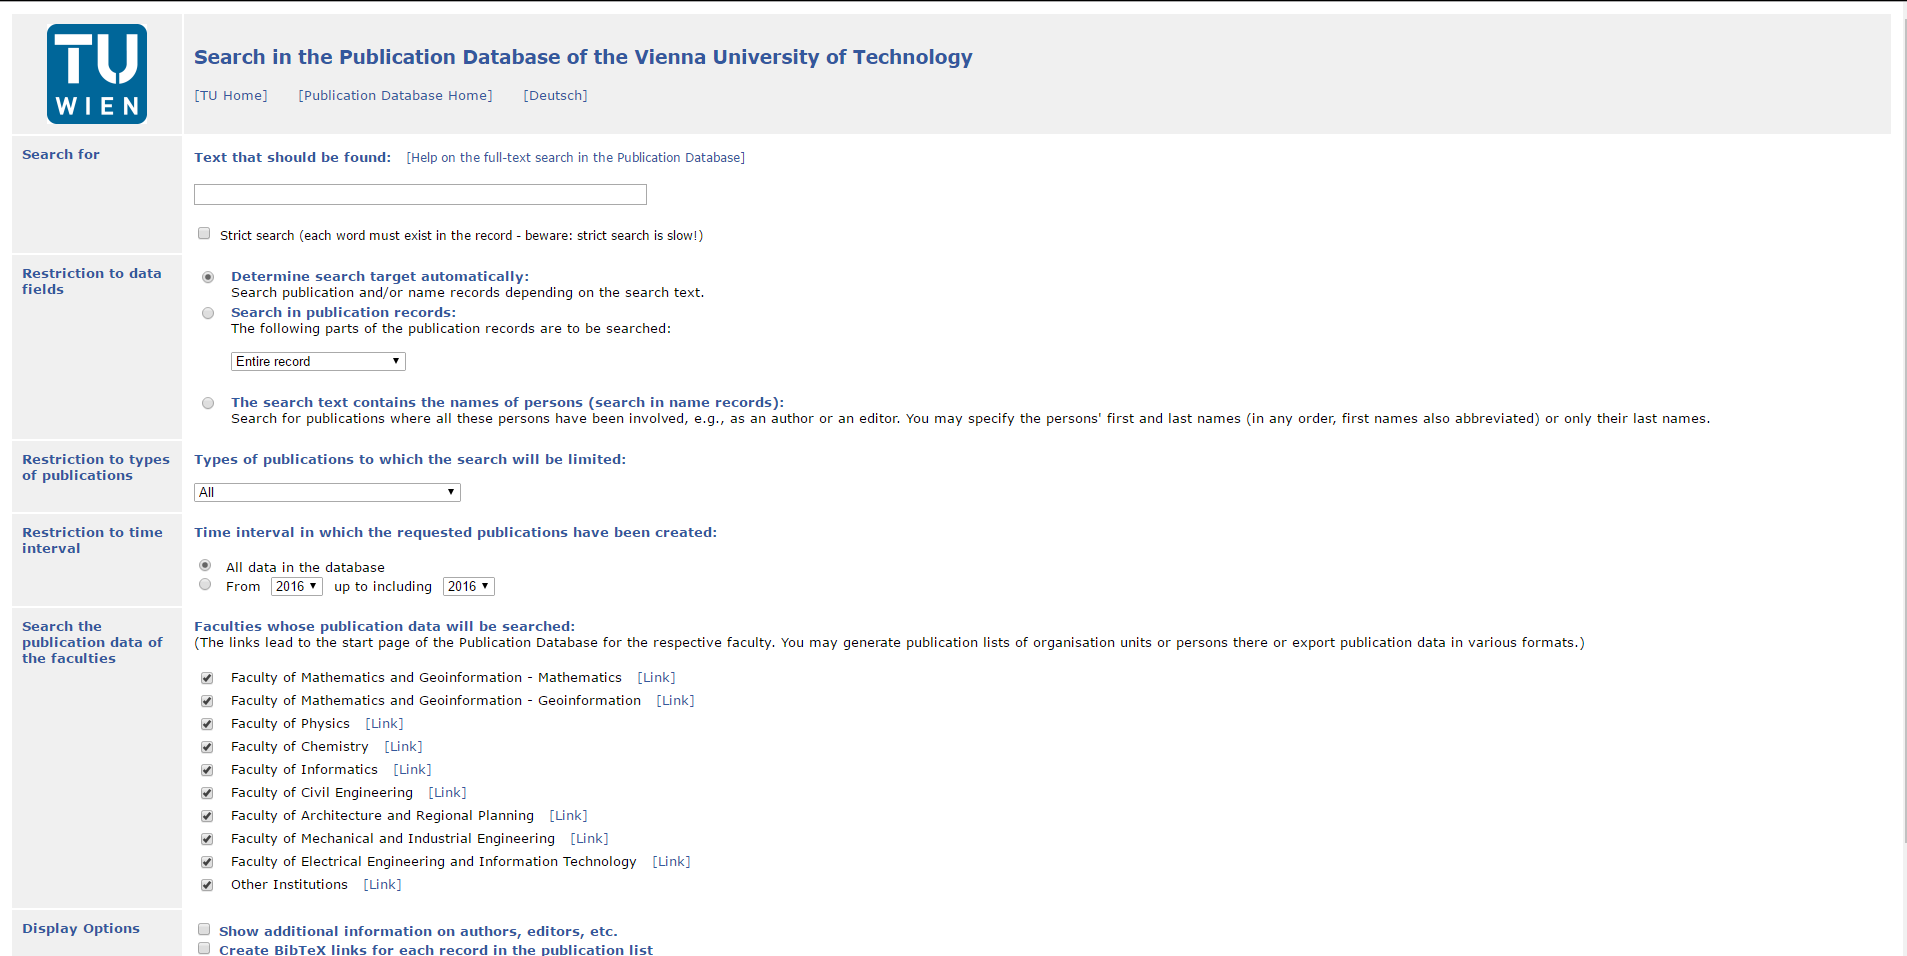
\includegraphics{images/screenshots/screenshot_pub_database.PNG}}}
\caption[Publication database]{Publication database}
\label{Fi:pub_db}
\end{figure}

\paragraph{Use case}\label{section:pub_db_usecase}
The proposed use case applied to the already existing publication database of the university. In the current state the database can be accessed via its website~\footnote{\url{www.publik.tuwien.ac.at/pubstart.php}}, where an interface for search exists. For other search parameters a request to the administration has to be made. The introduced LOD approach provides an LOD interface to the existing database, so the data can be accessed over e.g. SPARQL. This use case follows the principle of the existing ``Open Research Online''~\footnote{\url{http://data.open.ac.uk/page/context/oro}} endpoint from the Open University, which expose information about publications originating from OU researchers using the BIBO Ontology (see section~\ref{subsubsec:ontologies} for details).

\paragraph{Statistically evaluation}
Similar to the library use case the interviewees liked the idea and found it all ``extremely useful''. Everyone could imagine such a project at TUVienna and would also use it.

\begin{figure}[htbp]
\centering
	\begin{tikzpicture}
		\begin{axis}		
			[title=Usefulness of publication data as LOD,
			ybar,% Balken
			% urspr�ngliche y-Werte unterhalb der Balken:
			nodes near coords,
			nodes near coords align=above,
			point meta=rawy,
			axis x line=bottom, axis y line=left,% Achsen nur unten und links,
			%xlabel=blub,ylabel=bla, % Beschriftung der Achsen
			ymin=0,% minimaler y-Wert ist 0
			xtick=data,% xticks nur an Stellen mit Daten
			enlargelimits=auto,% Vergr��ern der R�nder des Diagramms
			% Ausgabe der x Werte ohne Tausendermarkierung@
			x tick label style={/pgf/number format/1000 sep=}]
			\addplot table[x=Question, y=Number] {data/data_publication_useful.csv};
		\end{axis}
	\end{tikzpicture}
		\begin{tikzpicture}
		\begin{axis}		
			[title=Imagine at TUVienna? Would use it?,,
			ybar,% Balken
			% urspr�ngliche y-Werte unterhalb der Balken:
			nodes near coords,
			nodes near coords align=above,
			point meta=rawy,
			axis x line=bottom, axis y line=left,% Achsen nur unten und links,
			%xlabel=blub,ylabel=bla, % Beschriftung der Achsen
			ymin=0,% minimaler y-Wert ist 0
			symbolic x coords = {No, Yes},
			xtick=data,% xticks nur an Stellen mit Daten
			enlargelimits=auto,% Vergr��ern der R�nder des Diagramms
			% Ausgabe der x Werte ohne Tausendermarkierung@
			x tick label style={/pgf/number format/1000 sep=},
			legend pos=north west]
			\addplot table[x=Answer, y=Imagine] {data/data_publication_use.csv};
			\addplot table[x=Answer, y=Use] {data/data_publication_use.csv};
			\legend{Can imagine, Would use}
		\end{axis}
	\end{tikzpicture}
	\caption[Usefulness of publication data]{Usefulness of publication data as LOD}\label{Fi:pub-data}
\end{figure}

\paragraph{Needs, potential benefits}
In contrast to the previous use case, the work amount of work was significant lesser stated, because the data are already there, just as the need of being up-to-date of the database.\newline 
Further some of the interviewed persons (independent to each other) come up with the idea of building an application based on the Linked Open Data interface to provide an overview of a researcher references as a widget or similar for a personal website. The data could be interlinked e.g. with the LOD interface of the Springer publisher~\footnote{\url{www.lod.springer.com/}} and complemented by including the Journal Impact Factor (JIF).

\paragraph{Barriers, potential disadvantages}
The interviewees identified uniformly a problem with the data ownership. Although there is an administration of the database, the \textit{ownership} of the data itself is very unclear and therefore a contact and responsible person would be hard to find for such a project - there needs to be more investigation.\newline
Another point, some of the interviewed persons were concerned of, was quality assurance - to use the data, they need to be synchronized with the original database. To taking care of this point, the implementation of a similar project has to ensure this.

\subsubsection{Other data}
\%\%\%\%tbd\%\%\%\%
\paragraph{Needs, potential benefits, use-cases}
\paragraph{Challenges}
